% %%% Change aspectratio to 16:9
% \setlength\pdfpagewidth{16.00cm}%
% \setlength\textwidth{16.00cm}%
% \setlength\pdfpageheight{9.00cm}%

\begin{frame}
  \frametitle{0. Régression polynomiale}
  \begin{itemize}
  \item[]
    $\dset = \{ (\xvec^i, y^i) \}_{i=1, \dots, n}$  \hspace{1em} $\xvec^i \in \RR^p$ \hspace{0.5em} $y^i \in \RR$
  \item Nous savons apprendre un modèle de la forme $(x_1, x_2, \dots, x_p) \mapsto \beta_0 + \beta_1 x_1 + \beta_2 x_2 + \dots \beta_p x_p$ \blue{(régression linéaire)}
  \item Comment apprendre un modèle de la forme $(x_1, x_2, \dots, x_p) \mapsto \beta_0 + \beta_1 x_1 + \beta_2 x_2 + \dots \beta_p x_p + \beta_{11} x_1^2 + \beta_{12} x_1 x_2 + \dots + \beta_{pp} x_p^2$ ?
    \pause
  \item[] Nouvelle représentation : $\varphi: (x_1, x_2, \dots, x_p) \mapsto (1, x_1, x_2, \dots, x_p, x_1^2, x_1x_2, \dots, x_p^2) \in \RR^m$ \hspace{0.5em} $m = \frac{(p+1)(p+2)}{2}$
  \item[] Une fonction linéaire de $\varphi(\xvec)$ est une fonction quadratique de $\xvec$ \blue{(régression quadratique)}
  \item Se généralise à tout degré $d$ en créant $\binom{p+d}{p}$ variables \blue{(régression polynomiale)}
  \end{itemize}
\end{frame}

\begin{frame}
  \frametitle{1. Généralisation et surapprentissage}
  \begin{itemize}
  \item \red{Généralisation :} capacité du modèle à \blue{faire de bonnes
      prédictions sur des données dont on ne connaît pas l'étiquette}
  \item \blue{Défi principal} de l'apprentissage supervisé : le \red{surapprentissage} \textcolor{gray!70}{(overfitting)}
    \begin{itemize}
    \item i.e. la performance est meilleure sur les données d'apprentissage que sur de nouvelles données 
    \item \black{Plutôt facile :} entraîner un modèle qui prédise bien sur les données d'apprentissage
    \item[] Surtout avec \blue{beaucoup de paramètres}
    \item \black{Difficile :} garantir qu'il prédise bien sur de nouvelles données
    % \item[] Exemple extrême : \blue{apprentissage \frquote{par c\oe{}ur}}
    \item[] Exemple extrême : \blue{apprentissage « par c\oe{}ur »}
    \end{itemize}
  \end{itemize}
\end{frame}

\begin{frame}
  \frametitle{1. Généralisation et surapprentissage}
  \begin{itemize}
  \item \blue{données} $\dset = \{ (\xvec^i, y^i) \}_{i=1, \dots, n}$ 
  \item \blue{hypothèses}
    \begin{itemize}
    \item $(\xvec^i, y^i)$ réalisation de $(X_i, Y_i)$ i.i.d et de même
      distribution que $(X, Y)$
    \item  $Y = \Phi(X) + \varepsilon$
    \end{itemize}
  \item Le surapprentissage vient de la difficulté à ne pas capturer le \red{bruit} $\varepsilon$ en approchant $\Phi$
    \begin{itemize}
    \item \red{bruit de mesure}
  \item \red{bruit d'étiquetage}
  \item \red{insuffisance du modèle}
  \end{itemize}
  \end{itemize}
\end{frame}    

\begin{frame}
  \frametitle{1. Généralisation et surapprentissage}
  \begin{center}
    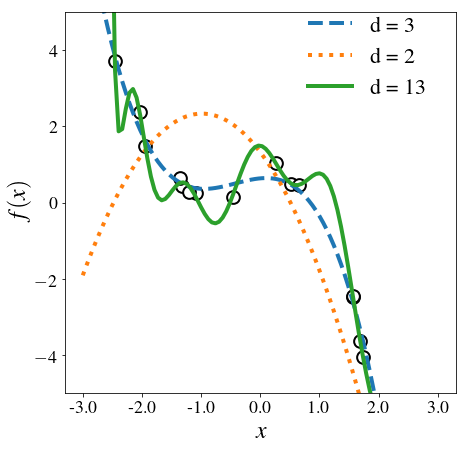
\includegraphics[width=.5\textwidth]{figures/overfit_regr}
  \end{center}
\end{frame}

\begin{frame}
  \frametitle{2. Erreur de généralisation}
  \begin{itemize}
  \item \red{Erreur de généralisation} : erreur \blue{sur de nouvelles données} du modèle $\hat{f}_{\dset}$ appris sur $\dset$ 
  \item Formellement : $\EE[L(Y, \hat{f}_{\dset}(X))]$ 
  \item En pratique, \blue{estimée} en 
    \blue{mettant de côté} une partie des données :
    \begin{itemize}
    \item On sépare les données en un \red{jeu d'entraînement} et un \red{jeu de test} (typiquement, 80\%--20\%)
    \pause
    \begin{center}
      \begin{tikzpicture}
        \draw [draw=MyBlue, thick] (0.,5.5) rectangle (10.,4.5) node[pos=.5]{\blue{Jeu de données}};
        \draw [->, draw=MyDarkGrey, line width=1.5] (5, 4.3) -- (5, 3.8);
        \draw [draw=MyDarkGrey, thick] (0.,3.5) rectangle (8.,2.5) node[pos=.5]{\black{Entraînement}};
        \draw [draw=MyDarkGrey, thick] (8.,3.5) rectangle (10.,2.5)  node[pos=.5]{\black{Test}};
      \end{tikzpicture}
    \end{center}
    \item Le \red{jeu d'entraînement} \textcolor{gray!70}{(train set)} sert à apprendre le modèle
    \item Le \red{jeu de test} sert à estimer l'erreur de généralisation du modèle
    \end{itemize}
  \end{itemize}
\end{frame}

\begin{frame}
  \frametitle{Règle d'or}
  \begin{center}
    \red{NE PAS TOUCHER au jeu de test} \\ sauf pour évaluer l'erreur de généralisation du modèle
  \end{center}
\end{frame}

\begin{frame}
  \frametitle{2. Erreur de généralisation}
  \begin{itemize}
  \item La \red{validation croisée} \textcolor{gray!70}{(cross-validation)} permet :
    \begin{itemize}
    \item d'utiliser toutes les données pour l'entraînement et pour la validation
    \item d'obtenir une performance moyenne (+/- écart-type)  moins sensible au choix du jeu de test
    \end{itemize}
  \item On sépare le jeu de données en K \blue{blocs} \textcolor{gray!70}{(folds)}
    \begin{itemize}
    \item[] En pratique, K=5 ou K=10 le plus souvent (équilibre entre le nombre
      d'expériences et la taille de chaque jeu d'entraînement)
    \end{itemize}
  \item On utilise tour à tour chacun des blocs comme \blue{jeu de
      validation} et l'union des autres comme \blue{jeu d'entraînement}
  \item[$\Rightarrow$] K erreurs $\rightarrow$ \blue{erreur de généralisation} du modèle
  \end{itemize}
\end{frame}

\begin{frame}
  \frametitle{Validation croisée}
  \begin{center}
    \small
    \begin{tikzpicture}
      \draw [draw=MyBlue, thick] (0, 6.5) rectangle (7.5, 6) node[pos=.5]{\blue{Jeu de données}};
      \pause
      \draw [->, draw=MyDarkGrey, line width=1.5] (3.75, 5.9) -- (3.75, 5.4);
      \draw [draw=MyDarkGrey, thick] (0.,5.3) rectangle (1.5,4.8) node[pos=.5]{\black{Bloc 1}};
      \draw [draw=MyDarkGrey, thick] (1.5,5.3) rectangle (3.,4.8) node[pos=.5]{\black{Bloc 2}};
      \draw [draw=MyDarkGrey, thick] (3.,5.3) rectangle (4.5,4.8) node[pos=.5]{\black{Bloc 3}};
      \draw [draw=MyDarkGrey, thick] (4.5,5.3) rectangle (6.,4.8) node[pos=.5]{\black{Bloc 4}};
      \draw [draw=MyDarkGrey, thick] (6.,5.3) rectangle (7.5,4.8) node[pos=.5]{\black{Bloc 5}};
      \pause
      \draw [->, draw=MyDarkGrey, line width=1.5] (3.75, 4.7) -- (3.75, 4.2);
      \draw [draw=MyDarkGrey, thick] (0.,4.1) rectangle (1.5,3.6) node[pos=.5]{\black{Test 1}};
      \draw [draw=MyDarkGrey, thick] (1.5,4.1) rectangle (7.5,3.6) node[pos=.5]{\black{Entraînement 1}};
      \pause
      \draw [->, draw=MyOrange, thick] (7.7, 3.85) -- (8.2, 3.85) node[pos=2.3]{\red{Erreur 1}};
      \pause
      \node[text width=1em] at (3.75, 3.3) {$\boldsymbol{\vdots}$};
      \draw [draw=MyDarkGrey, thick] (0.,2.8) rectangle (6,2.3) node[pos=.5]{\black{Entraînement 5}};
      \draw [draw=MyDarkGrey, thick] (6.,2.8) rectangle (7.5,2.3) node[pos=.5]{\black{Test 5}};
      \draw [->, draw=MyOrange, thick] (7.7, 2.55) -- (8.2, 2.55) node[pos=2.3]{\red{Erreur 5}};
      \pause
      \draw [decorate, decoration = {brace}, draw=MyOrange, line width=2] (9.5, 3.9) --  (9.5,2.4);
      \node[text width=6em] at (10.9, 3.2) {\red{Erreur de \\généralisation}};
    \end{tikzpicture}
  \end{center}
  \begin{itemize}
  \item[] \only<6>{L'erreur moyenne sur les K folds est une estimation de l'erreur de généralisation du modèle entraîné sur l'ensemble des données.}
  \end{itemize}
\end{frame}

\begin{frame}[t]
  \frametitle{3. Critères de performance (classification)}
  \begin{itemize}
  \item \red{Pourcentage d'erreur :} proportion d'observations mal classifiées
    \pause
  \item \black{Problème :} cas où les classes ne sont \blue{pas équilibrées}
    \begin{itemize}
    \item[] \black{Exemple :} détection de fraude
    \item 99\% des observations ne sont pas des fraudes
    % \item Un modèle qui prédit toujours \frquote{non} a un pourcentage d'erreur de 1\%.
    \item Un modèle qui prédit toujours « non » a un pourcentage d'erreur de 1\%.
    \end{itemize}
    \pause
  \item \red{Matrice de confusion} \textcolor{gray!70}{(confusion matrix)}
  \end{itemize}
  \begin{center}
    \small
      \only<3>{
        \begin{tabular}[h]{|lc|c|c|} \hline
          & & \multicolumn{2}{|c|}{Classe réelle} \\ \cline{3-4}
          & & 0 & 1 \\ \hline
          Classe & \multicolumn{1}{|c|}{0} & Vrais Négatifs (TN) & Faux Négatifs (FN) \\ \cline{2-4}
          prédite & \multicolumn{1}{|c|}{1} & Faux Positifs (FP) & Vrais Positifs (TP) \\ \hline
        \end{tabular}}
      \only<4>{
        \textcolor{gray!70}{\begin{tabular}[h]{|lc|c|c|} \hline
          & & \multicolumn{2}{|c|}{True class} \\ \cline{3-4}
          & & 0 & 1 \\ \hline
          Predicted & \multicolumn{1}{|c|}{0} & True Negatives (TN) & False Negatives (FN) \\ \cline{2-4}
          class & \multicolumn{1}{|c|}{1} & False Positives (FP) & True Positives (TP) \\ \hline
        \end{tabular}}}
  \end{center}
\end{frame}

\begin{frame}
  \frametitle{3. Critères de performance (classification)}
  \begin{center}
    {\small \begin{tabular}[h]{|lc|c|c|c|} \hline
      & & \multicolumn{2}{|c|}{Classe réelle} & \\ \cline{3-4}
      & & 0 & 1 & \\ \hline
      Classe & \multicolumn{1}{|c|}{0} & Vrais Négatifs (TN) & Faux Négatifs (FN) & {\color{MyOrange}{TN+FN}} \\ \cline{2-5}
      prédite & \multicolumn{1}{|c|}{1} & Faux Positifs (FP) & Vrais Positifs (TP) & {\color{MyOrange}{TP+FP}} \\ \hline
       &  & {\color{Aubergine}{TN + FP}} & {\color{Aubergine}{TP + FN}} & \\ \hline
    \end{tabular}}
  \end{center}

  \begin{itemize}
  \item Sensibilité \textcolor{gray!70}{(sensitivity)} = rappel \textcolor{gray!70}{(recall)} = taux de vrais positifs = $\frac{\text{TP}}{\color{Aubergine}{\text{TP + FN}}}$
  \item Spécificité \textcolor{gray!70}{(specificity)} = taux de vrais négatifs \textcolor{gray!70}{(TN rate)} = $\frac{\text{TN}}{\color{Aubergine}{\text{TN + FP}}}$
  \item Précision \textcolor{gray!70}{(precision)} = $\frac{\text{TP}}{\color{MyOrange}{\text{TP + FP}}}$
  \item Précision \textcolor{gray!70}{(accuracy)} = $\frac{\text{TP + TN}}{\text{TP + FP + TN + FN}}$
  \item Score F \textcolor{gray!70}{(F-score)} = moyenne harmonique (précision, rappel) = $\frac{\text{2 TP}}{\color{MyOrange}{\text{TP + FP}} {\color{MyDarkGrey}{\text{ + }}} \color{Aubergine}{\text{TP + FN}}}$
  \end{itemize}
\end{frame}

\begin{frame}
  \frametitle{3. Critères de performance (classification)}
  \begin{minipage}[h]{0.5\linewidth}
    \begin{itemize}
    \item[] \red{Courbe ROC} (Receiver-Operator Characteristic)
    \item Évaluer la \blue{fonction de décision} avant qu'elle ne soit seuillée
    \item \blue{Choisir} le seuil de décision 
    \item Résumé : \red{aire sous la courbe ROC} (AUC, AUROC)
    \end{itemize}
  \end{minipage}
  \hfill
  \begin{minipage}[h]{0.45\linewidth}
    \begin{center}
      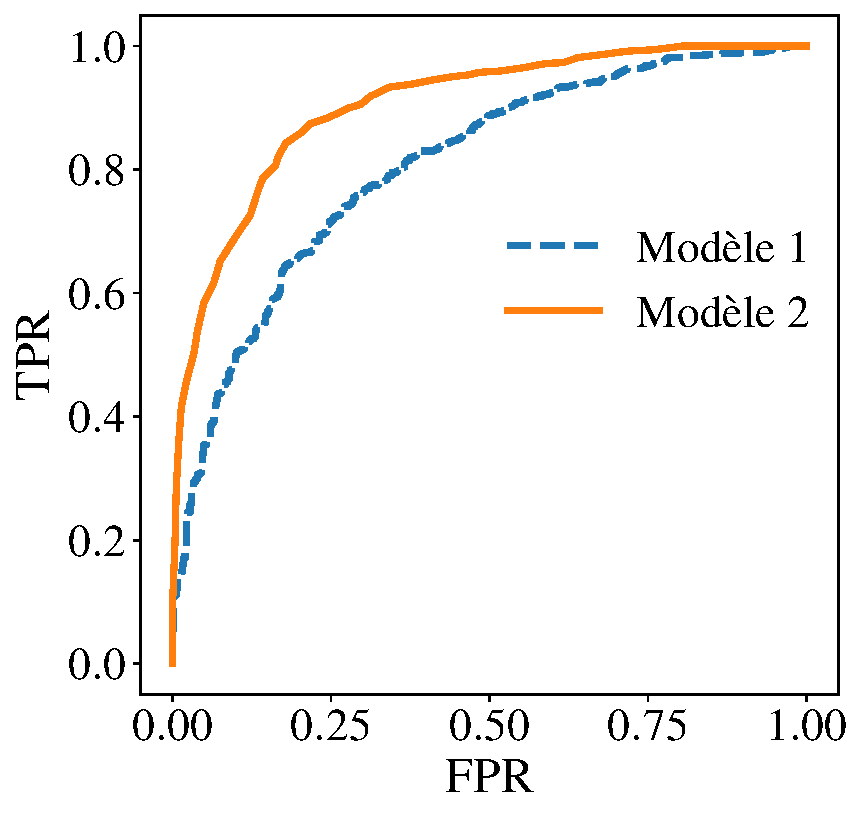
\includegraphics[width=\textwidth]{figures/roc_curve}  
    \end{center}
  \end{minipage}
  {\small TPR = True Positive Rate = $\frac{\text{TP}}{\text{P}}$ = sensibilité \hspace{2em}
  FPR = False Positive Rate = $\frac{\text{FP}}{\text{N}}$ = 1 - spécificité}
\end{frame}

\begin{frame}
  \frametitle{3. Évaluation d'un modèle (régression)}
  \begin{itemize}
  \item \blue{Compter} le nombre d'erreurs n'a pas de sens
    \pause
  \item Somme des carrés des erreurs : $\text{RSS} = \sum_{i=1}^n \left(y_i - f(\xvec_i) \right)^2$
  \item \tikzmark{ml0}{Racine} de l'erreur quadratique moyenne \textcolor{gray!70}{(Root Mean Squared Error)} : 
    \[\text{RMSE} = \sqrt{\frac1n \sum_{i=1}^n \left(y_i - f(\xvec_i) \right)^2}\]
  \item \tikzmark{ml1}{Corrélation de Pearson}  :
    \[
      R^2 = \frac{\sum_{i=1}^n \left( y_i - \overline{y} \right) \left( f(\xvec_i) - \overline{f(\xvec)} \right) }{\sqrt{\sum_{i=1}^n \left(y_i - \overline{y} \right)^2} \sqrt{\sum_{i=1}^n \left(f(\xvec_i) - \overline{f(\xvec)} \right)^2}}
    \]
  \end{itemize}
\end{frame}

\begin{frame}
  \frametitle{4. Régularisation}
  \begin{itemize}
  \item Par principe, la \blue{minimisation du risque empirique} conduit facilement au \blue{surapprentissage}
  \item La \red{régularisation} consiste à \blue{contraindre} le problème de MRE pour
    \blue{limiter la complexité} du modèle
    \begin{itemize}
    \item \red{Complexité $\Omega(f)$} d'un modèle $f$ : notion théorique, par ex. Vapnik--Chervonenkis
    \item Intuitivement : \blue{flexibilité} des modèles que l'on peut apprendre
    \item Proxys  : nombre de paramètres ; amplitude possible de ces paramètres
    \end{itemize}
    \[ \hat{f} = \argmin_{f \in \fcal} \frac1n \sum_{i=1}^n L(y_i, f(\xvec_i))
      {\color{MyOrange} \, + \, \lambda \, \Omega(f) } \hspace{1em} \lambda > 0
    \]
  \end{itemize}
\end{frame}

\begin{frame}
  \frametitle{Coefficient de régularisation}
  \[ \hat{f} = \argmin_{f \in \fcal} \frac1n \sum_{i=1}^n L(y_i, f(\xvec_i))
    {\color{MyOrange} \, + \, \lambda \, \Omega(f) } \hspace{1em} \lambda > 0
  \]
  \begin{itemize}
  \item \red{Coefficient de régularisation} $\lambda > 0$ :
     gouverne l'importance relative entre la
    minimisation du risque empirique et la complexité $\Omega(f)$ du modèle.
  \end{itemize}
  
  \begin{itemize}
  \item $\lambda = 0$ :
  \item $\lambda \to +\infty$ :
  \end{itemize}
\end{frame}

\begin{frame}
  \frametitle{4. Régularisation}
  \begin{itemize}
  \item Exemple 1 : \red{Régularisation ridge} (ou \red{$\ell_2$}, ou \red{weight decay})
    \begin{itemize}
    \item Pour un modèle paramètrique de paramètres $\theta_1, \theta_2, \dots, \theta_m$,
    \item[] $\Omega(\thetavec) = \ltwonorm{\thetavec}^2 = \sum_{j=1}^m \theta_j^2$ contrôle \blue{l'amplitude des paramètres} 
      \pause
      \vspace{1em}
    \item \red{Régression (linéaire) ridge :}
      \[\argmin_{\betavec \in \RR^{p+1}} \frac1n 
        \left(\yvec - X \betavec \right)^\top \left(\yvec - X \betavec
        \right) + \lambda \ltwonorm{\betavec}^2 \]
    \item[] Admet toujours une unique solution
      $\betavec^* = \left(X^\top X + \lambda I_p \right)^{-1} X^\top \yvec$
      car ajouter une matrice diagonale à coefficients strictement positifs à
      $X^\top X$ la rend inversible
    \end{itemize}
  \end{itemize}
\end{frame}

\begin{frame}
  \frametitle{4. Régularisation }
  \begin{itemize}
  \item Exemple 2 : \red{Régularisation $\ell_1$} 
    \begin{itemize}
    \item Pour un modèle paramètrique de paramètres $\theta_1, \theta_2, \dots, \theta_m$,
    \item[]
      $\Omega(\thetavec) = \lonenorm{\thetavec} = \sum_{j=1}^m \lvert \theta_j
      \rvert$ contrôle \blue{le nombre de paramètres non nuls} $\rightarrow$
      \red{parcimonie} \textcolor{gray!70}{(sparsity)} \pause \vspace{1em}
    \item \red{Lasso} (Least Absolute Sparse Selection Operator) :
      \[\argmin_{\betavec \in \RR^{p+1}} \frac1n 
        \left(\yvec - X \betavec \right)^\top \left(\yvec - X \betavec
        \right) + \lambda \lonenorm{\betavec} \]
    \item Pas de solution analytique 
    \end{itemize}
  \end{itemize}
\end{frame}

\begin{frame}
  \frametitle{4. Régularisation}
  \black{Chemins de régularisation :} Chaque courbe correspond à une variable
  
  \begin{minipage}[t]{0.45\linewidth}
    \vspace{0pt}
    \begin{center}
      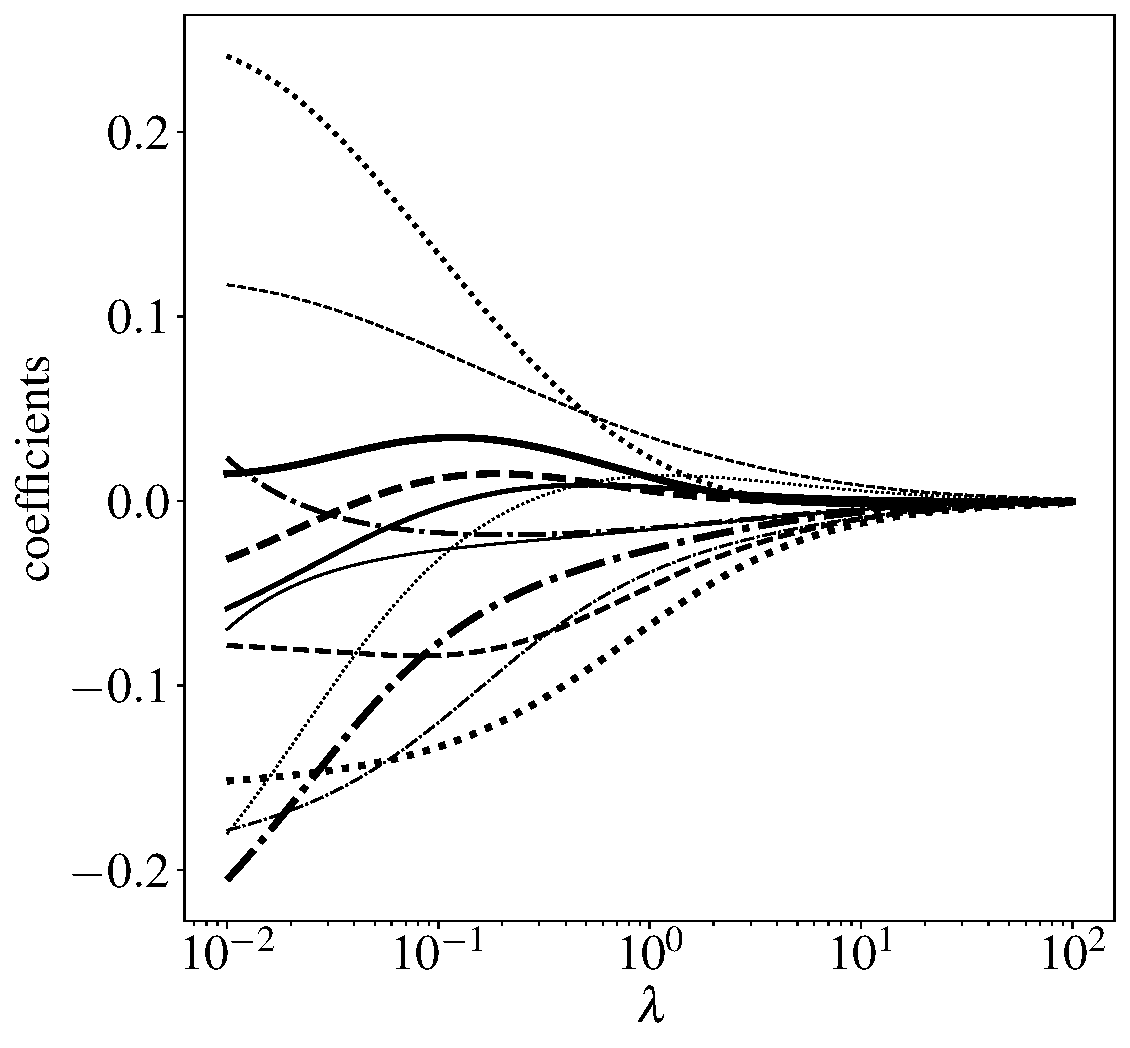
\includegraphics[width=\textwidth]{figures/ridge_path}
      Ridge
    \end{center}
  \end{minipage}%
  \hfill
  \begin{minipage}[t]{0.45\linewidth}
    \vspace{0pt}
    \begin{center}
      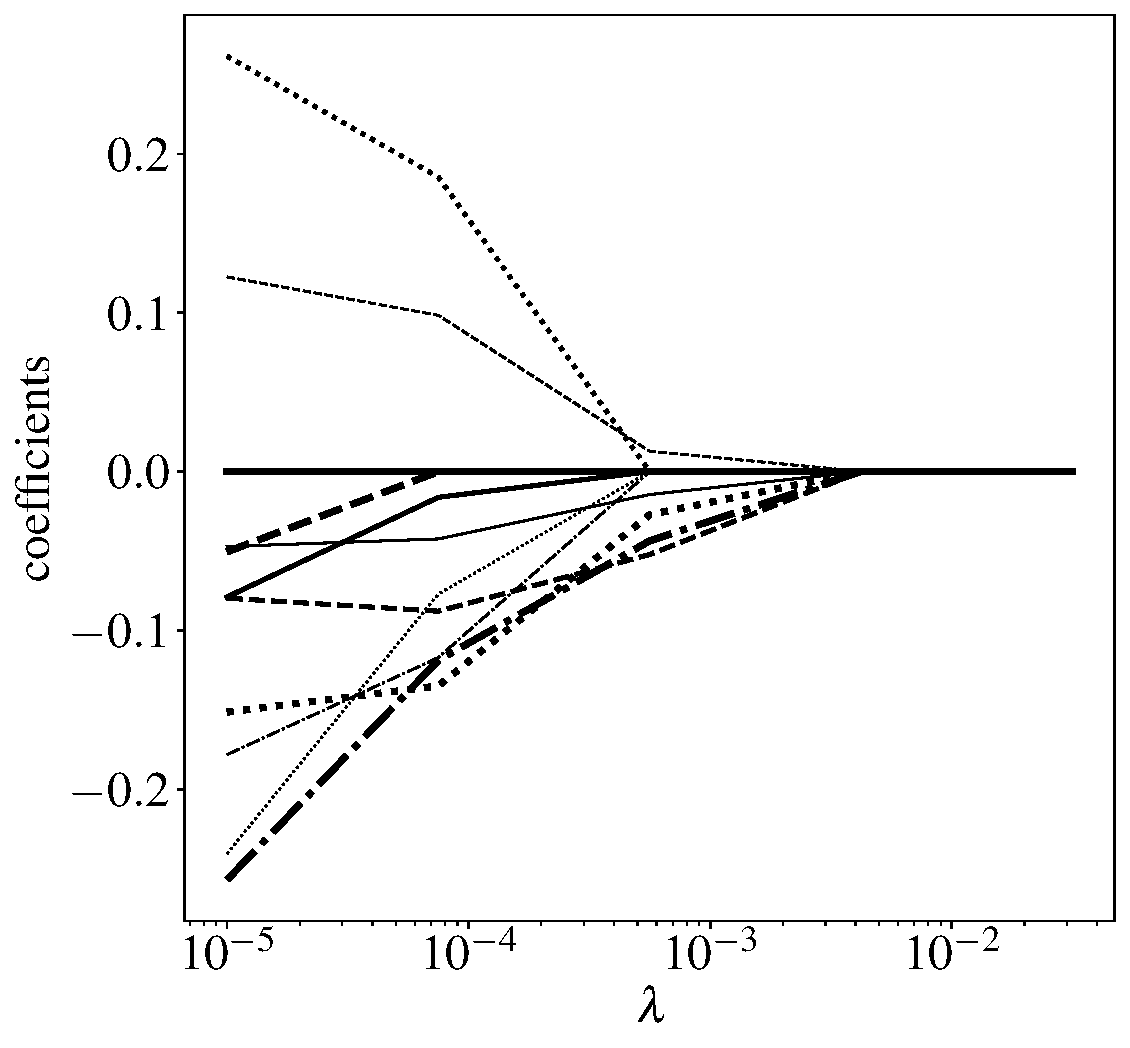
\includegraphics[width=\textwidth]{figures/lasso_path}
      Lasso
    \end{center}
  \end{minipage}
\end{frame}

\begin{frame}[t]
  \frametitle{4. Régularisation}
  \black{Point de vue du compromis biais-variance}
  \begin{itemize}
  \item[] $\dset = \{ (\xvec^i, y^i) \}_{i=1, \dots, n}$ \hspace{1em}  $(\xvec^i, y^i)$ réalisation de $(X_i, Y_i)$ copies i.i.d de $(X, Y)$ 
    $Y = \Phi(X) + \varepsilon$
  \item Pour une observation $\xvec$ : $f(\xvec)$ est la réalisation de $F$ estimateur de $\Phi(\xvec)$ \\
   $F$ est une fonction de $(X_1, X_2, \dots, X_n, Y_1, Y_2, \dots Y_n)$
 \item \blue{EQM} de $F$ : $\EE[(F - \Phi(\xvec))^2] = \text{Biais}(F) + \text{Var}(F)$ \blue{(compromis biais-variance)}
 \item \blue{Régularisation :}  \blue{réduire l'EQM} en \blue{biaisant} le modèle de sorte à \blue{réduire sa variance}\\
   (variance $\equiv$ complexité)
  \end{itemize} 
\end{frame}

\begin{frame}
  \frametitle{4. Régularisation}
  \black{Point de vue géométrique}

  \begin{minipage}[t]{0.45\linewidth}
    \vspace{0pt}
    \begin{center}
      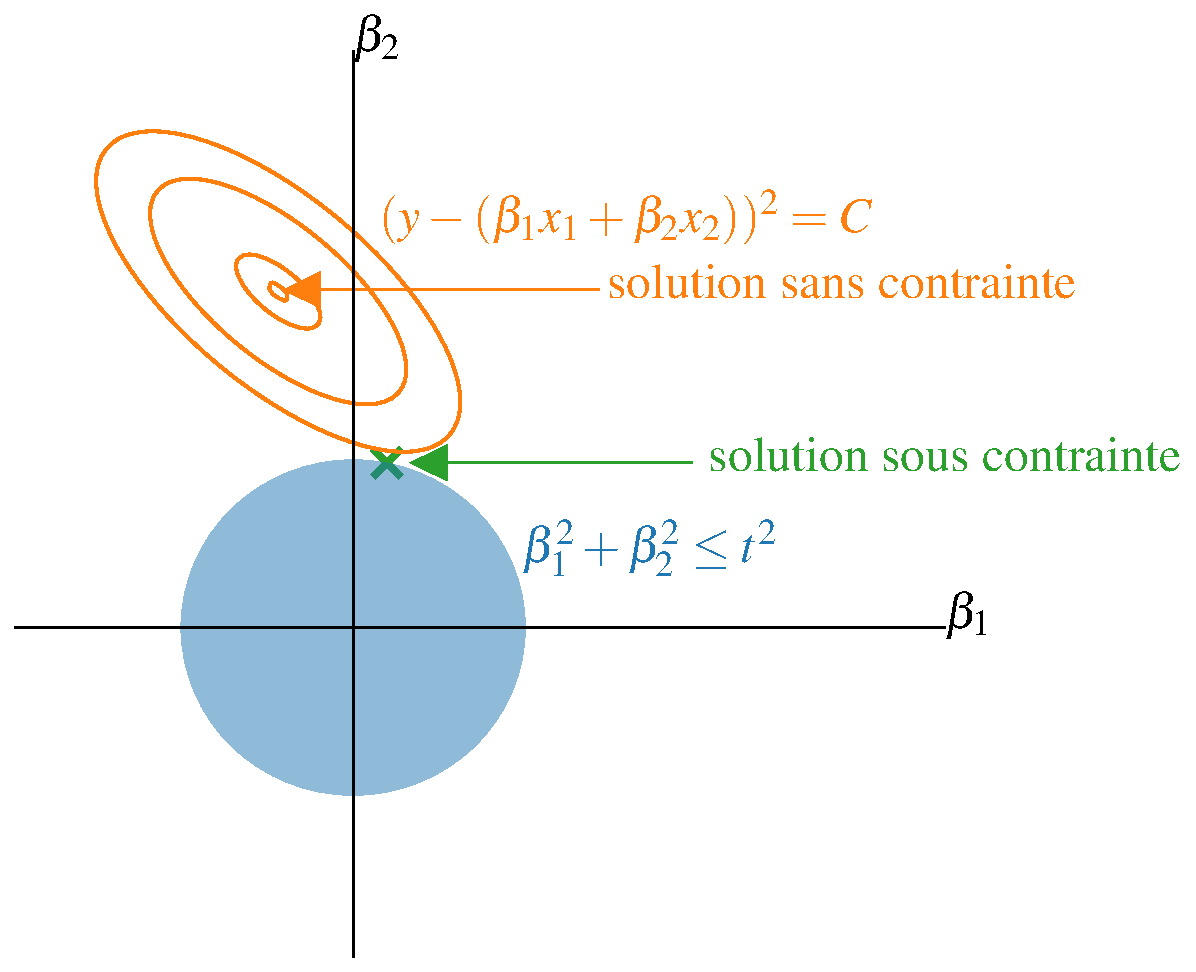
\includegraphics[width=\textwidth]{figures/l2reg}
      Régularisation $\ell_2$
    \end{center}
  \end{minipage}%
  \hfill
  \begin{minipage}[t]{0.45\linewidth}
    \vspace{0pt}
    \begin{center}
      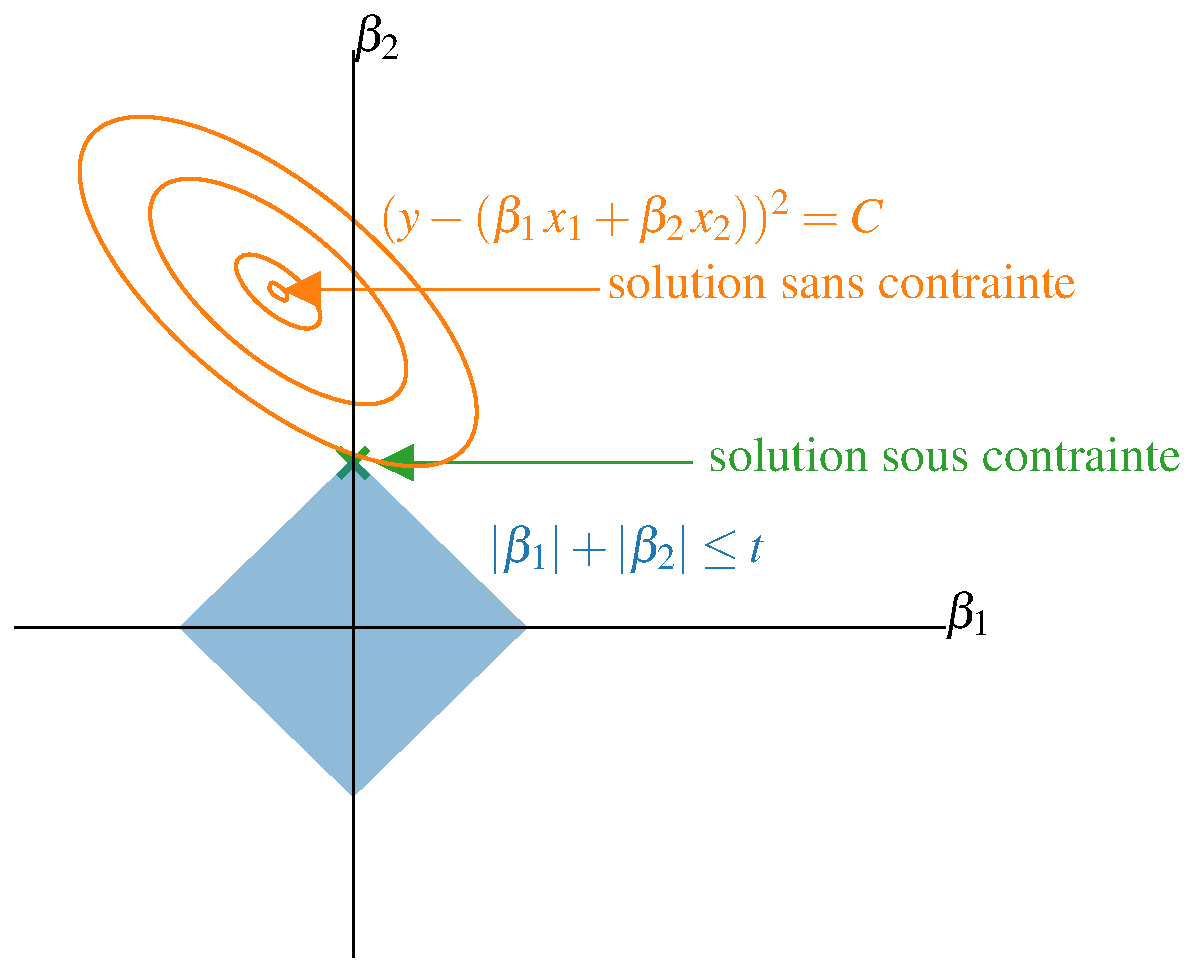
\includegraphics[width=\textwidth]{figures/l1reg}
      Régularisation $\ell_1$
    \end{center}
  \end{minipage}
  
\end{frame}

\begin{frame}
  \frametitle{4. Régularisation}
  \black{Point de vue de l'estimation statistique}
  
  % \begin{minipage}[t]{0.45\linewidth}
  %   \vspace{0pt}
    \begin{itemize}
    \item[] Sous hypothèse de bruit gaussien $Y = \Phi(X) + \varepsilon$
      \hspace{1em} $\varepsilon \sim \ncal(0, \sigma^2)$
    \item MRE $\equiv$
      estimation des paramètres du modèle par maximum de vraisemblance
    \item \blue{MRE + régularisation $\ell_2$} $\equiv$ estimation des paramètres du
      modèle par maxium a posteriori, avec une prior \blue{gaussienne}
    \item \blue{MRE + régularisation $\ell_1$} $\equiv$ estimation des paramètres du
      modèle par maxium a posteriori, avec une prior \blue{de Laplace}
    \end{itemize}
  % \end{minipage}%
  % \hfill
  % \begin{minipage}[t]{0.45\linewidth}
  %   \vspace{0pt}
    \begin{center}
      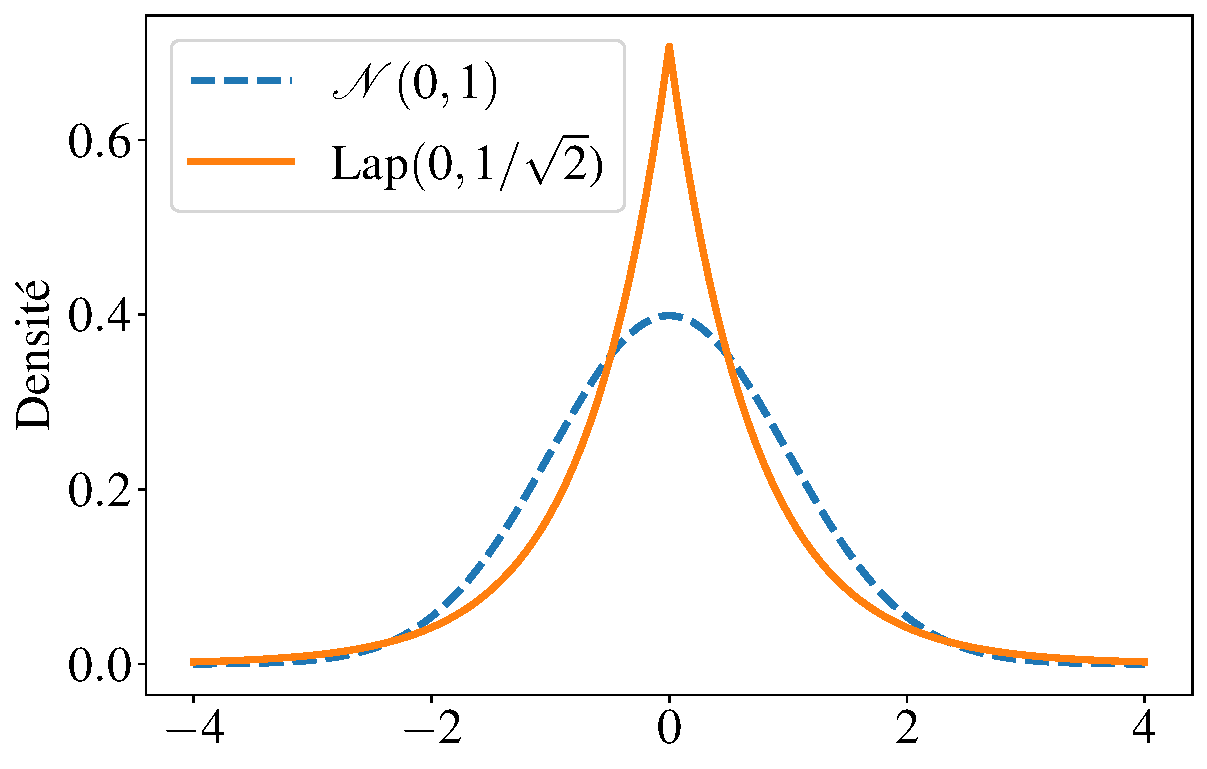
\includegraphics[width=0.45\textwidth]{figures/laplace_vs_gauss}  
    \end{center}
  % \end{minipage}
\end{frame}



\begin{frame}
  \frametitle{4. Régularisation}
  \black{Elastic Net}
  \begin{itemize}
  \item Variables \blue{corrélées} : le Lasso sélectionne l'une d'entre elles aléatoirement
  \item[$\Rightarrow$] \blue{instabilité}
  \item \red{Elastic Net}
    \[
      \Omega(\thetavec) = \alpha \ltwonorm{\thetavec}^2 + (1-\alpha) \lonenorm{\thetavec} \hspace{1em} 0 < \alpha < 1       \]
    \end{itemize}
\end{frame}

\begin{frame}
  \frametitle{5. Sélection de modèle}
  \begin{itemize}
  \item \red{Hyperparamètre :} paramètre \blue{de l'algorithme d'apprentissage} et non pas du modèle
    \begin{itemize}
    \item Un hyperparamètre \blue{définit} le problème de minimisation du
      risque empirique
    \item Un paramètre est \blue{déterminé} (= \blue{appris}) par la résolution du problème de minimisation du risque empirique 
    \end{itemize}
  \item Ex :
    \begin{itemize}
    \item \blue{Coefficient de régularisation} $\lambda$
    \item \blue{Degré} $d$ d'une régression polynomiale.
    \end{itemize}
  \end{itemize}
\end{frame}


\begin{frame}[t]
  \frametitle{5. Sélection de modèle}
  \black{Recherche sur grille} \textcolor{gray!70}{(grid search)}
  \begin{itemize}
  \item On cherche l'\blue{hyperparamètre} qui donne \blue{la meilleure performance} sur le jeu de \blue{test.}
    \[
      \text{Ex :} \, \widehat{\lambda} \in \argmin_{\lambda > 0} \frac{1}{n_{\text{test}}} \sum_{i=1}^{n_{\text{test}}} \text{Err}
      \left(y^i, \widehat{f}_{\lambda}(\xvec^i) \right) ;\]\[ 
      \widehat{f}_{\lambda} \in \argmin_{f \in \fcal} \frac{1}{n_{\text{train}}} \sum_{i=1}^{n_{\text{train}}} L(y_i, f(\xvec_i)) \, + \, \lambda \, \Omega(f)        
    \]
  \pause
  \item En pratique :
    \begin{itemize}
    \item On teste une \blue{grille} (liste) prédéfinie de valeurs de l'hyperparamètre
    \item[] Ex : $\lambda \in [10^{-3}, 10^{-2}, 10^{-1}, 1, 10, 10^{2}, 10^{3}]$ 
    \item Plus grande liberté sur le choix de Err que de $L$
    \end{itemize}
  \end{itemize}
\end{frame}

\begin{frame}
  \frametitle{5. Sélection de modèle}
  \black{Plusieurs hyperparamètres}

  \begin{minipage}[t]{0.46\linewidth}
    \vspace{0pt}
    \begin{center}
      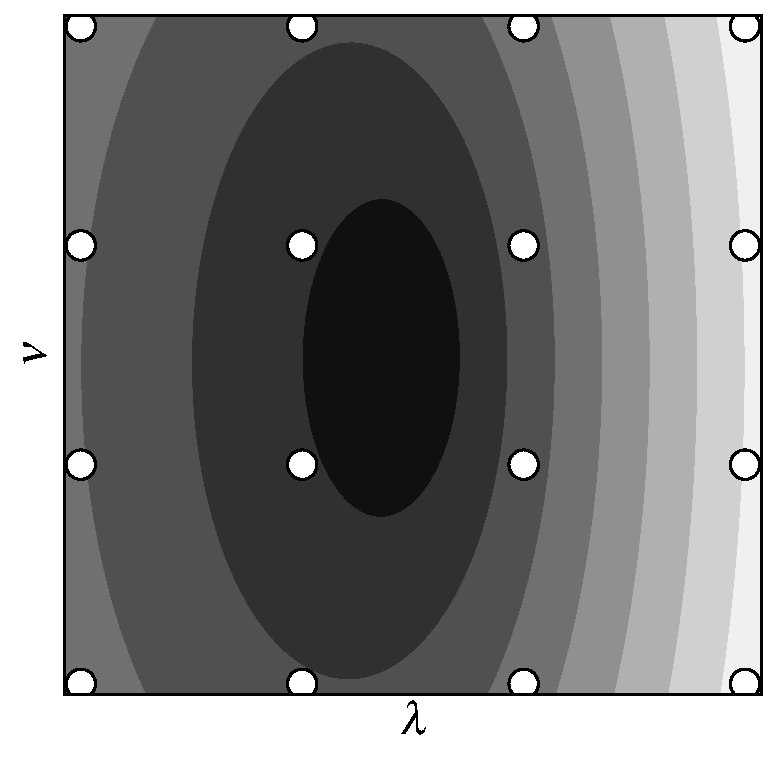
\includegraphics[width=0.9\textwidth]{figures/grid_search}
      Recherche sur grille \textcolor{gray!70}{(grid search)}
    \end{center}
  \end{minipage}%
  \hfill
  \begin{minipage}[t]{0.46\linewidth}
    \vspace{0pt}
    \begin{center}
      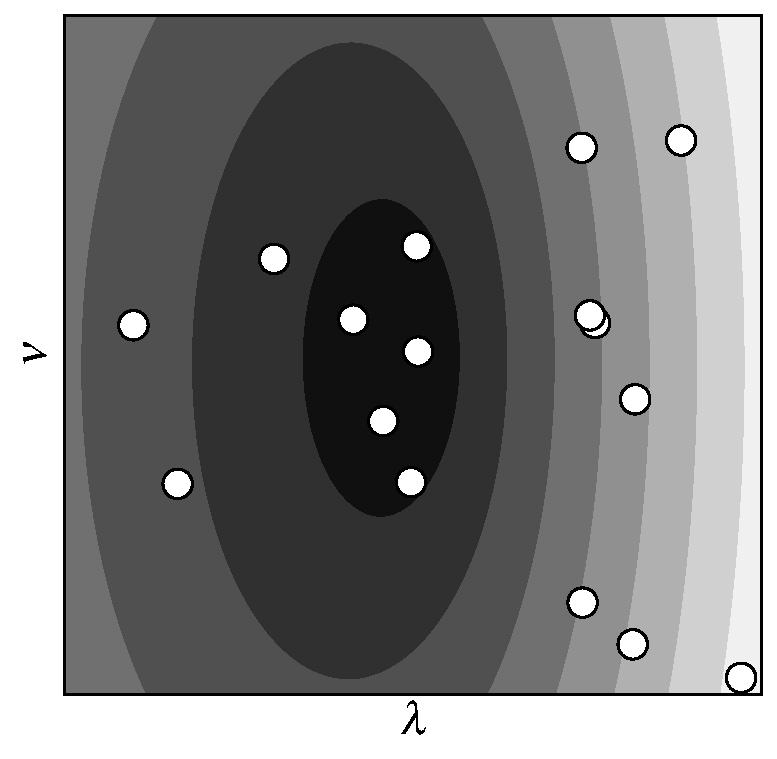
\includegraphics[width=0.9\textwidth]{figures/random_search}
      Recherche aléatoire \textcolor{gray!70}{(random search)}
    \end{center}
  \end{minipage}
\end{frame}



\begin{frame}
  \frametitle{5. Sélection de modèle}
  \begin{itemize}
  \item Pour déterminer \blue{le meilleur modèle} parmi ceux appris :
    \begin{itemize}
    \item avec différents algorithmes d'apprentissage ;
    \item avec différentes valeurs d'hyperparamètre(s) pour le même algorithme 
    \end{itemize}
  \item \black{Idée :} sélectionner celui qui a la \blue{meilleure performance sur le jeu de test.}
    \pause
  \item \black{Attention :} on ne peut plus utiliser le jeu de test pour déterminer l'\blue{erreur de
      généralisation !} 
  \pause
  \item On sépare les données en 3 jeux : apprentissage, \red{validation} et test.
  \end{itemize}
  \begin{center}
    \begin{tikzpicture}[scale=0.8]
      \small
      \draw [draw=MyBlue, thick] (0.,5.5) rectangle (10.,4.5) node[pos=.5]{\blue{Jeu de données}};
      \pause
      \draw [->, draw=MyDarkGrey, line width=2] (5, 4.3) -- (5, 3.8);
      \draw [draw=MyDarkGrey, thick] (0.,3.5) rectangle (5.5,2.5) node[pos=.5]{\black{Entraînement}};
      \draw [draw=MyDarkGrey, thick] (5.5,3.5) rectangle (8.,2.5) node[pos=.5]{\black{Validation}};
      \draw [draw=MyDarkGrey, thick] (8.,3.5) rectangle (10.,2.5)  node[pos=.5]{\black{Test}};
    \end{tikzpicture}
  \end{center}
\end{frame}

\begin{frame}
  \begin{center}
  \frametitle{5. Sélection de modèle}
    \begin{tikzpicture}
      \draw [draw=MyDarkGrey, thick] (0.,3.5) rectangle (5.5,2.5) node[pos=.5]{\black{Entraînement}};
      \draw [draw=MyDarkGrey, thick] (5.5,3.5) rectangle (8.,2.5) node[pos=.5]{\black{Validation}};
      \draw [draw=MyDarkGrey, thick] (8.,3.5) rectangle (10.,2.5)  node[pos=.5]{\black{Test}};
    \end{tikzpicture}
  \end{center}
  \begin{itemize}
  \item Le \red{jeu d'entraînement} sert à apprendre \blue{chacun des} modèles
  \item Le \red{jeu de validation} sert à \blue{sélectionner} le meilleur modèle
  \item Le \red{jeu de test} sert à estimer l'erreur de généralisation \blue{du modèle sélectionné}
  \pause
  \item \black{Problèmes :}
    \begin{itemize}
    \item On utilise seulement une fraction des données pour l'entraînement
    \item Possiblité que le modèle sélectionné ait une meilleure performance
      sur ce jeu de validation précis à cause d'un artefact.
    \end{itemize}
  \end{itemize}
\end{frame}

\begin{frame}
  \frametitle{5. Sélection de modèle}
  \black{Validation croisée (sélection de modèle)}
  \begin{itemize}
    \setlength{\itemsep}{3pt}
  \item On peut aussi utiliser la \blue{validation croisée} pour la \blue{sélection de modèle}
  \item On sépare le jeu d'entraînement en K \blue{blocs} (ou folds)
  \item Pour chaque algorithme ou valeur d'hyperparamètre à évaluer :
    \begin{itemize}
    \item On utilise tour à tour chacun des blocs comme \blue{jeu de
        validation} et l'union des autres comme \blue{jeu d'entraînement}
  \item[$\Rightarrow$] on obtient K scores de performance $\rightarrow$ \blue{performance moyenne} 
  \end{itemize}
\item On sélectionne l'algorithme ou la valeur d'hyperparamètre qui donne la meilleure performance moyenne
\item On réentraîne sur le jeu d'entraînement l'algorithme sélectionné
\item On estime l'erreur de généralisation en évaluant sur le jeu de test le modèle ainsi obtenu
  \end{itemize}
\end{frame}

\begin{frame}
  \frametitle{5. Sélection de modèle}
  \black{Validation croisée (sélection de modèle)}
    \begin{center}
    \small
    \begin{tikzpicture}
      \draw [draw=MyBlue, thick] (0.,7.7) rectangle (9.,7.2) node[pos=.5]{\blue{Jeu de données}};
      \pause
      \draw [->, draw=MyBlue, line width=1.5] (4.5, 7.1) -- (4.5, 6.6);
      \draw [draw=MyDarkGrey, thick] (0, 6.5) rectangle (7.5, 6)  node[pos=.5]{\black{Entraînement}};      
      \draw [draw=MyDarkGrey, thick] (7.5, 6.5) rectangle (9, 6) node[pos=.5]{\black{Test}};      
      \pause
      \draw [->, draw=MyDarkGrey, line width=1.5] (3.75, 5.9) -- (3.75, 5.4);
      \draw [draw=MyDarkGrey, thick] (0.,5.3) rectangle (1.5,4.8) node[pos=.5]{\black{Bloc 1}};
      \draw [draw=MyDarkGrey, thick] (1.5,5.3) rectangle (3.,4.8) node[pos=.5]{\black{Bloc 2}};
      \draw [draw=MyDarkGrey, thick] (3.,5.3) rectangle (4.5,4.8) node[pos=.5]{\black{Bloc 3}};
      \draw [draw=MyDarkGrey, thick] (4.5,5.3) rectangle (6.,4.8) node[pos=.5]{\black{Bloc 4}};
      \draw [draw=MyDarkGrey, thick] (6.,5.3) rectangle (7.5,4.8) node[pos=.5]{\black{Bloc 5}};
      \pause
      \draw [->, draw=MyDarkGrey, line width=1.5] (3.75, 4.7) -- (3.75, 4.2);
      \draw [draw=MyDarkGrey, thick] (0.,4.1) rectangle (1.5,3.6) node[pos=.5]{\black{Val 1}};
      \draw [draw=MyDarkGrey, thick] (1.5,4.1) rectangle (7.5,3.6) node[pos=.5]{\black{Entraînement 1}};
      \pause
      \draw [->, draw=MyOrange, thick] (7.7, 3.85) -- (8.2, 3.85) node[pos=2.3]{\red{Erreur 1}};
      \pause
      \node[text width=1em] at (3.75, 3.3) {$\boldsymbol{\vdots}$};
      \draw [draw=MyDarkGrey, thick] (0.,2.8) rectangle (6,2.3) node[pos=.5]{\black{Entraînement 5}};
      \draw [draw=MyDarkGrey, thick] (6.,2.8) rectangle (7.5,2.3) node[pos=.5]{\black{Val 5}};
      \draw [->, draw=MyOrange, thick] (7.7, 2.55) -- (8.2, 2.55) node[pos=2.3]{\red{Erreur 5}};
      \pause
      \draw [decorate, decoration = {brace}, draw=MyOrange, line width=2] (9.5, 3.9) --  (9.5,2.4);
      \node[text width=6em] at (10.9, 3.2) {\red{Erreur moyenne}};
      \pause
      \draw [draw=MyPink, thick] (-0.1, 5.4) rectangle (12.2, 2.2) node[pos=0.32, below=60]{\color{MyPink}{Pour chaque algorithme/valeur d'hyperparamètre}};
      \pause
      \node[align=left] at (4., 1.5) {\color{MyPink}{$\rightarrow$ meilleur algorithme/valeur d'hyperparamètre}};
      \pause
      \draw [->, draw=MyPink, line width=2] (7.3, 1.7) -- (7.3, 5.9);
      \draw [draw=MyPink, line width=2, fill=MyLightGrey] (0, 6.5) rectangle (7.5, 6) node[pos=.5]{\color{MyPink}{\textbf{Ré-entraînement }}};      
      \pause
      \draw [draw=MyOrange, line width=2] (7.5, 6.5) rectangle (9, 6) node[pos=.5]{\red{Test}};      
      \draw [->, draw=MyOrange, thick] (9.1, 6.25) -- (9.6, 6.25) node[pos=5.1]{\red{Erreur de généralisation}};
    \end{tikzpicture}
  \end{center}    
\end{frame}

% \begin{frame}
%   \frametitle{5. Sélection de modèle}
%   \black{Validation croisée imbriquée}
%   \begin{itemize}
%   \item Utiliser une validation croisée :
%     \begin{itemize}
%     \item pour \blue{la sélection de modèle} (boucle interne)
%     \item et pour \blue{l'évaluation} du modèle sélectionné (boucle externe)
%     \end{itemize}
%   \item Peut devenir \blue{coûteux en calculs :}
%     \begin{itemize}
%     \item \textbf{Exemple :} si K = 5 pour la boucle interne, K=10 pour la boucle externe, et on a
%       10 valeurs d'hyperparamètre à évaluer : 500 modèles à entraîner.
%     \item Cependant, facile à paralléliser.
%     \end{itemize}
%   \end{itemize}
% \end{frame}


\begin{frame}
  \frametitle{Références / page pub}
  \begin{itemize}
  \item \black{Introduction au Machine Learning}, Chloé-Agathe Azencott, Dunod InfoSup \\
    Version électronique (PDF) sans exercices disponible gratuitement sur  \textcolor{MyBlue}{\href{https://cazencott.info/index.php/pages/Introduction-au-Machine-Learning}{http://cazencott.info [lien cliquable]}}\\
  \item \black{Le Machine Learning avec scikit-learn}, Aurélien Géron, Dunod
    InfoSup
  \item \blue{MOOC scikit-learn } \textcolor{MyBlue}{\href{https://inria.github.io/scikit-learn-mooc/}{[lien cliquable]}}
  \end{itemize}
\end{frame}

% %%% Change aspectratio back to 128:96
% \setlength\pdfpagewidth{12.80cm}%
% \setlength\pdfpageheight{9.60cm}%
